\chapter{Hardware inerciální jednotky}

\begin{figure}[h]
    \centering
    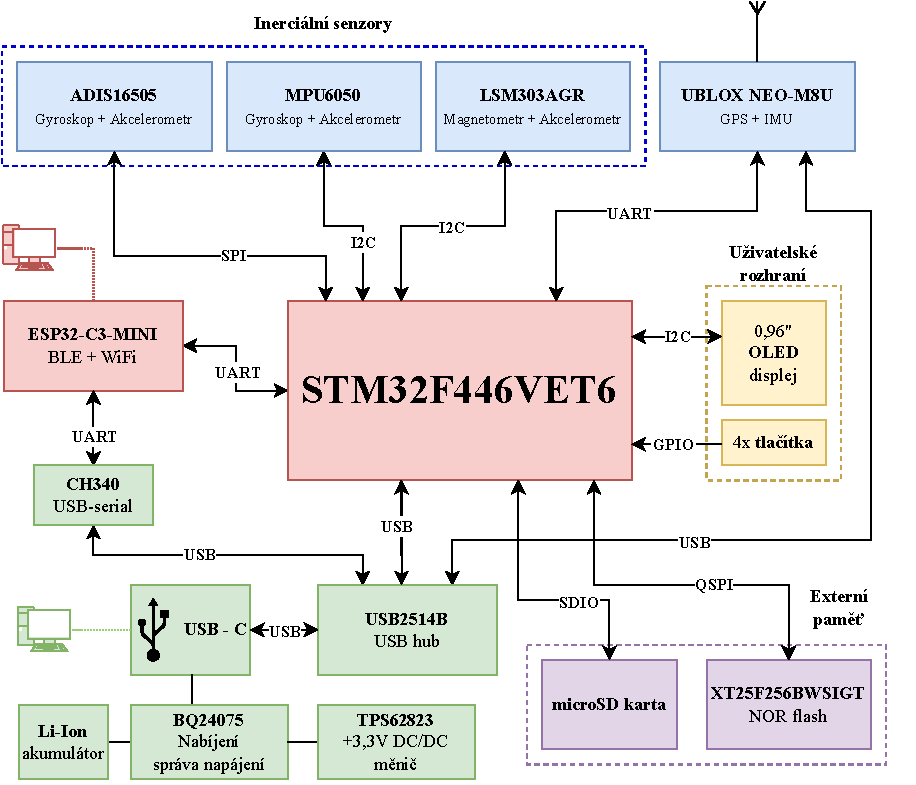
\includegraphics[width=\textwidth]{obrazky/IMUnav_H00_block}
    \caption{Blokové schéma inerciální jednotky}
\end{figure}

Hardware inerciální jednotky je realizován tak, aby umožňoval zaznamenávat hodnoty změřené inerciálními senzory a poskytovat dohromady data o rozměru 9~DoF (akcelerometr, gyroskop a magnetometr). Jednotka také obsahuje GPS modul s vestavěným IMU, jehož použití by mohlo být vhodné například v prostorech s alespoň částečným pokrytím signálu GPS.

Naměřená data je možné uložit do externí NOR Flash paměti připojené k MCU, popřípadě lze využít i kartu typu microSD. K přenosu dat pro jejich následné zpracování v PC primárně slouží ESP32-C3, umožňující bezdrátovou komunikaci přes Wifi, nebo Bluetooth. Konektor USB typu C umožňuje nabíjení vestavěného Li-Ion akumulátoru jednotky a komunikaci mezi PC a ESP32, GPS modulem a hlavním MCU skrze vestavěný USB rozbočovač. Toto rozhraní je plánované pro použití např. ke konfiguračním, nebo ladícím účelům.

Pro jednoduchou volnost pohybu je jednotka napájena jedním Li-Ion akumulátorem velikosti 18650, při záznamu dat tedy nebude potřeba externího zdroje energie. Grafický OLED displej a 4 tlačítka slouží jako uživatelské rozhraní při používání jednotky.

\section{Akcelerometr a gyroskop} \label{AccGyroText}
Jednotka obsahuje dvě 6~DoF IMU (gyroskop s akcelerometrem) rozdílných parametrů a řádově rozdílné ceny. Takto odlišné součástky byly vybrány proto, aby bylo možné porovnat vliv přesnosti, šumu, biasu a driftu senzorů na následně zpracovaná data.
V tabulce \ref{table:fyzikalniPorovnaniIMU} jsou porovnány důležité parametry senzorů MPU6050 a ADIS16505-2. Pro účely inerciální navigace je důležitý zejména nízký bias a drift senzorů, aby při integraci dat k vyhodnocení polohy nebyla integrována i driftová chyba, což má za výsledek velmi nepřesné zpracování hodnot.

\begin{table}[h!]
\centering
\begin{tabular}{c||c c c}
\hline 
Model IMU & MPU6050 & ADIS16505-2 & jednotka \\ 
\hline
\hline 
\multicolumn{4}{c}{Parametry gyroskopů} \\
\hline
\hline
Dynamický rozsah  & \makecell{programovatelný, \\ $\pm 250$, $\pm 500$, \\$\pm 1000$, $\pm 2000$} & $\pm 500$ & $\SI[per-mode = symbol]{}{\degree\per\second}$ \\ 
\hline 
Citlivost  \tablefootnote{Pro porovnání citlivosti byl vybrán dynamický rozsah $\SI[per-mode = symbol]{500}{\degree\per\second}$ senzoru MPU6050 pro možnost porovnání hodnoty s druhým senzorem} & $65,5$ & $2621440$ & $\SI[per-mode = symbol]{}{\LSB\per(\degree\per\second)}$ \\ 
\hline 
Drift v ose x a z & $\pm 20$ & $\pm 0,14$ & $\SI[per-mode = symbol]{}{\degree\per\second}$ \\ 
\hline 
Drift v ose y & $\pm 20$ & $\pm 1,4$ & $\SI[per-mode = symbol]{}{\degree\per\second}$ \\ 
\hline 
\makecell{Efektivní hodnota hustoty \\šumu při 10Hz pro osy x a y} & 0,005 & 0,0043 & $\SI{}{\degree\per\second\per\sqrt{\Hz}}$ \\ 
\hline 
\makecell{Efektivní hodnota hustoty \\šumu při 10Hz pro osu z} & 0,005 & 0,0034 & $\SI{}{\degree\per\second\per\sqrt{\Hz}}$ \\ 
\hline 
\hline 
\multicolumn{4}{c}{Parametry akcelerometrů} \\
\hline
\hline
Dynamický rozsah  & \makecell{programovatelný, \\ $\pm 19,6$, $\pm 39,2$, \\$\pm 78,4$, $\pm 156,8$} & $\pm 78,4$ & $\SI[per-mode = symbol]{}{\metre\per\second\squared}$ \\ 
\hline 
Citlivost  \tablefootnote{Pro porovnání citlivosti byl vybrán dynamický rozsah $\SI[per-mode = symbol]{78,4}{\metre\per\second\squared}$ senzoru MPU6050 pro možnost porovnání hodnoty s druhým senzorem} & $418$ & $26756268$ & $\SI[per-mode = symbol]{}{\LSB\per(\metre\per\second\squared)}$ \\ 
\hline 
Drift v ose x a y & $\pm 0,491$ & $\pm 0,0196$ & $\SI[per-mode = symbol]{}{\metre\per\second\squared}$ \\ 
\hline 
Drift v ose z & $\pm 0,785$ & $\pm 0,0196$ & $\SI[per-mode = symbol]{}{\metre\per\second\squared}$ \\ 
\hline 
\makecell{Efektivní hodnota hustoty \\šumu při 10Hz pro osy x a y} & 3924 & 167 & $\SI{}{\micro\metre\per\second\squared\per\sqrt{\Hz}}$ \\ 
\hline 
\makecell{Efektivní hodnota hustoty \\šumu při 10Hz pro osu z} & 3924 & 243 & $\SI{}{\micro\metre\per\second\squared\per\sqrt{\Hz}}$ \\ 
\hline 

\end{tabular} 
\caption{Porovnání základních parametrů gyroskopů \cite{euxR3Yh5ol4JWNAi} \cite{UZFqHmQU7ZzI3OLB}} 
\label{table:fyzikalniPorovnaniIMU}
\end{table} 


Integrovaný obvod MPU6050 je standardní 6 osé MEMS IMU, vhodné mimo jiné pro použití v mobilních zařízeních a dalších podobných aplikacích. Jeho vnitřní gyroskop a akcelerometr má softwarově přepínatelné rozsahy měřených veličin. Kromě inerciálních senzorů má i vestavěný signálový procesor pro fúzi a filtrování dat přímo v integrovaném obvodu. Tato funkce může být vhodná pro odlehčení výpočetního výkonu hlavního procesoru, ovšem pro účely této práce nebude signálový procesor využit, jelikož se měřená data budou zpracovávat až po jejich naměření v PC, ne v reálném čase. Vzorkovací frekvence gyroskopu je 8 kHz a akcelerometru 1 kHz, oba senzory mají 16bitové rozlišení.
\cite{euxR3Yh5ol4JWNAi}

MPU6050 disponuje rozhraním I2C s maximální frekvencí hodinového signálu 400 kHz. \cite{euxR3Yh5ol4JWNAi}
Pokud bychom chtěli vyčítat ze senzoru data při maximální možné vzorkovací frekvenci, byla by potřeba minimální přenosová rychlost sběrnice:
\begin{equation}
f_{\mathrm{clk}}=3~\mathrm{osy} \times(f_{\mathrm{gyro}} + f_{\mathrm{acc}})\times (\mathrm{16bitů} + 2 \times \mathrm{ACK})=3\times(8000+1000)\times(16+2)=\SI{486}{\kilo\hertz}
\end{equation}
Při vyčítání dat o maximální vzorkovací frekvenci jsme omezeni samotným I2C rozhraním senzoru (využití maximální vzorkovací frekvence je teoreticky možné krátkodobě, pomocí interního 1kB FIFO zásobníku).\cite{euxR3Yh5ol4JWNAi}

Jelikož pro účely inerciální navigace stačí vzorkovací frekvence dat v  řádu stovek~Hz \cite{Wei2022}, tak není tato limitace omezující. Senzor je propojen s hlavním MCU přes I2C sběrnici s frekvencí hodinového signálu 400 kHz a není sdílena s žádným jiným zařízením, aby bylo možné, v případě potřeby, využít maximální dostupný potenciál senzoru (i přestože je reálná potřeba vzorkovací frekvence nižší).

Integrovaný obvod ADIS16505-2 je precizní 6 osé MEMS IMU, vhodné pro použití v průmyslových a navigačních aplikacích s poměrně nízkým driftem a vysokou přesností. Na rozdíl od MPU6050 nemá přepínatelný dynamický rozsah, je fixně daný variantou součástky. Vzorkovací frekvence gyroskopu i akcelerometru je 2 kHz, oba senzory mají 32bitové rozlišení. S hlavním MCU komunikuje přes sběrnici SPI s maximální frekvencí hodinového signálu 2,1 Mhz. \cite{UZFqHmQU7ZzI3OLB} Pokud budeme chtít vyčítat data ze senzoru při maximální možné vzorkovací frekvenci, bude potřeba minimální přenosová rychlost sběrnice: 
\begin{equation}
f_{\mathrm{clk}}=3~\mathrm{osy} \times(f_{\mathrm{gyro}} + f_{\mathrm{acc}})\times \mathrm{32bitů}=3\times(2000+2000)\times 32=\SI{384}{\kilo\hertz}
\end{equation}
Nejsme tedy omezeni maximální frekvencí hodinového signálu a můžeme teoreticky využívat senzor i při nejvyšší možné rychlosti.

Výrobce prodává tento obvod ve variantě 100 pinového BGA čipu, ale i jako vývojovou desku osazenou senzorem a kolíkovou lištou pro jednodušší práci s osazením DPS. \cite{UZFqHmQU7ZzI3OLB} Hardware jednotky byl navržen tak, aby bylo možné využít jak samotný BGA čip, tak i hotový modul s konektorem.

\section{Magnetometr}
Vzhledem k tomu, že výběr komerčně dostupných 9 DoF (akcelerometr, gyroskop a magnetometr) je značně omezený, popřípadě součástky prodávané jako 9osé IMU jsou ve skutečnosti moduly více součástek na jedné desce, tak je ve výsledném obvodovém zapojení použit senzor magnetické indukce jakožto samostatná součástka. 

Přestože fúze dat z magnetometru může mít pozitivní dopady na zmenšení chyby trajektorie \cite{Tkhorenko2018}, jeho použití uvnitř budov je značně omezené vzhledem k jednoduché ovlivnitelnosti měření blízkými feromagnetickými látkami, silovými rozvody elektřiny a pod. Proto nebyly na výběr magnetometru kladeny vysoké požadavky a slouží spíše pro porovnání vlivu přítomnosti / absence naměřených dat z tohoto senzoru.

K tomuto účelu byl vybrán běžně dostupný obvod LSM303AGR, který kromě magnetometru v pouzdře obsahuje i akcelerometr, ten ovšem nebude pro potřeby práce využit, jelikož tuto funkci obstarávají součástky z kapitoly \ref{AccGyroText}.

Magnetometr komunikuje s hlavním MCU přes sběrnici I2C s maximální vzorkovací frekvencí 150 Hz, dynamickým rozsahem $ \pm \SI{4.915}{\milli\tesla} $ a 16bitovým rozlišením. \cite{RD5DwZcremhT6bgp}

\section{GNSS}
Zajímavou a uživatelsky přívětivou kombinaci GNSS a inerciální navigace poskytuje například firma u-blox s řadou modulů podporující funkci „dead reckoning“. Jedná se o navigační moduly s vestavěným IMU, určené zejména do oblasti automotive. Jejich typický příklad použití, dle výrobce, je navigace aut, kdy při běžném provozu je zafixovaný signál z GNSS a při výpadku signálu (vjezd do garáže, tunelu apod.) je navigace modulem stále poskytována na základě dat z IMU. \cite{DLQg9bT6V1GWKhxh}

Navigační modul u-blox NEO-M8U byl vybrán a implementován do obvodového zapojení inerciální navigační jednotky.
Výrobce udává, že modul zvládne odhadovat polohu po ztrátě signálu GNSS po dobu 60 s s typickou odchylkou 10 \% trajektorie. Dále také modul při zapnutí odpovídající funkce umí využít interní IMU ke zvýšení maximální rychlosti aktualizace polohy až na 30 Hz. Jeho využití v rámci této práce může být různé, například pro navigaci v místech s alespoň částečným pokrytím signálu GNSS. \cite{DLQg9bT6V1GWKhxh}

NEO-M8U umí využívat všechny světové navigační systémy (uvedeny v tabulce~\ref{table:gnssBands})
\begin{table}[h!]
\caption{Podporované družicové systémy. \cite{DLQg9bT6V1GWKhxh} }
\centering
\begin{tabular}{c|c c }

GNSS systém & Pásmo & Frekvence (MHz) \\ 
\hline 
\hline
GPS & L1C/A & 1575,42 \\ 

GLONASS & L1OF & 1602 \\ 

BeiDou & B1 & 1561,098 \\ 

Galileo & E1-B/C & 1575,42 \\ 

\end{tabular} 

\label{table:gnssBands}
\end{table} 

Tento modul komunikuje s hlavním MCU přes sběrnici UART, pomocí standardizovaných NMEA příkazů v textové podobě, nebo pomocí binárního protokolu UBX, který je specifikován výrobcem. Použití protokolu NMEA je omezené pouze na standardní funkce GNSS modulů, pokud chceme využít speciálních funkcí, například inerciální navigace, je nutné použít proprietární protokol UBX. \cite{DLQg9bT6V1GWKhxh} NEO-M8U také disponuje USB portem, skrz který je možné modul ovládat a konfigurovat pomocí PC aplikace výrobce. Tento port je připojen na integrovaný USB rozbočovač a lze jej využít například pro vývojové účely.

\section{Paměť}
\begin{table}[h!]
\centering
\begin{tabular}{c|c}

Senzor & Odhadovaný bitrate \\ 
\hline 
\hline 
ADIS16505-2 & 375 kbit/s \\ 

MPU-6050 & 422 kbit/s \\ 

LSM303AGR & 7 kbit/s \\ 

NEO-M8U & 1 kbit/s \\ 
\hline

Celkem & 805 kbit/s (0,1MB/s) \\ 

\end{tabular} 
\caption{Odhad celkového bitratu pro záznam dat} 
\label{table:memoryBW}
\end{table} 
V případě, že bychom chtěli zaznamenávat data ze všech senzorů při jejich maximálních vzorkovacích frekvencích, nebude množství změřených dat zanedbatelné. V tabulce \ref{table:memoryBW} je hrubý odhad potřebné rychlosti záznamu dat pro tento krajní případ. Pokud bude měření trvat např. 2 minuty, vygenerujeme dohromady 12 MB dat, což převyšuje velikost paměti většiny dostupných MCU.

Z tohoto důvodu je v obvodovém zapojení inerciální jednotky implementována 32MB NOR Flash paměť, propojená s hlavním MCU přes sběrnici QUADSPI s maximální možnou hodinovou frekvencí 120 Mhz, měla by tedy být pro potřeby této aplikace dostačující. \cite{CgaRYSTpwKhEZZr7}

Kromě výše popsané Flash paměti jednotka obsahuje i slot na microSD kartu, která by z uživatelského hlediska mohla být jednodušší k použití, ovšem při zápisu může latence SD karty být (krátkodobě) až stovky ms \cite{Kraewinkel2020}. To by mohlo znemožnit její použití v případě, že by hlavní MCU měl nedostatek volné paměti RAM pro krátkodobé uchování dat, proto bude o její využití rozhodnuto až později.

\section{Uživatelské rozhraní}
\begin{figure}[h]
    \centering
    \includegraphics[width=0.3\textwidth]{obrazky/OLED}
    \caption{Fotografie grafického OLED displeje}
\end{figure}
Pro ovládání uživatelem disponuje jednotka grafickým OLED displejem s úhlopříčkou 0,96 palce a rozlišením $ 128 \times 64 $ pixelů, který je připojený přes sběrnici I2C. Společně s 4 tlačítky by měl poskytnout dostatečně univerzální a pohodlné uživatelské rozhraní.

\section{Napájení}
Inerciální jednotka je napájena z jednoho Li-Ion akumulátoru velikosti 18650. Nabíjení je realizováno obvodem BQ24075RGT, který monitoruje nabíjecí odebíraný proud jednotkou. Proud, kterým je nabíjen akumulátor je regulován tak, aby nepřekročil maximální hranici 900 mA z USB portu. \cite{F5eZCtr2LLRsr9NT}

Všechny součásti inerciální jednotky (až na RTC a zálohovací registry hlavního MCU a GPS modulu) jsou napájeny skrz DC/DC měnič z výstupního vývodu tohoto nabíjecího obvodu. V případě, že je připojena jednotka do USB a nabíjí se, na výstupním pinu nabíjecího obvodu je napájecí napětí USB portu. Díky tomu nedochází k velkým ztrátám pokud je jednotka zapnuta a nabíjí se zároveň. Jestliže je USB odpojeno, skrz interní tranzistor je jednotka napájena z akumulátoru. \cite{F5eZCtr2LLRsr9NT}

Nabíjecí obvod také umožňuje kompletní odpojení napájení jednotky přes jeden z vývodů. Toho je využito pro ochranu akumulátoru proti podvybití pomocí zapojení S/R klopného obvodu na napájení USB a jednoho z výstupů procesoru. Napětí akumulátoru je měřeno pomocí ADC mikrokontroléru. Jestliže klesne pod definovanou úroveň, pomocí pulzu bude celý obvod odpojen od napájení až do té doby, dokud uživatel znova nepřipojí jednotku do USB portu.

\begin{table}[h!]
\centering

\begin{tabular}{|c|c|}
\hline 
Součástka & Odhadovaný proud (mA) \\ 
\hline 
\hline 
STM32F446 & 50 \\ 
\hline 
ESP32 & 150 \\ 
\hline 
USB2514 & 135 \\ 
\hline 
ADIS16505 & 50 \\ 
\hline 
NEO-M8U & 30 \\ 
\hline 
OLED displej & 10 \\ 
\hline 
microSD karta & 50 \\ 
\hline 
\hline 
Celkem & 475 \\ 
\hline 
\end{tabular} 

\caption{Odhad spotřeby proudu 3,3V větve} 
\label{table:currentConsumption}
\end{table} 

Vzhledem k většímu počtu součástek není odebíraný proud z 3,3V napájecí větve malý (zhruba 0,5 A, viz. tabulka \ref{table:currentConsumption}). Budeme-li uvažovat rozsah výstupního napětí nabíjecího obvodu 3,5 V (vybitý akumulátor) až 5 V (zařízení připojené do USB) zjistíme, že pro napájení 3,3V větve není vhodný lineární regulátor, zejména kvůli vysokému ztrátovému výkonu. Ten je v krajním případě:

\begin{equation}
P_{\mathrm{ztrátový}} = (U_{\mathrm{USB}}-U_{\mathrm{IO}})\times I_{\mathrm{IO}}=(5-3,3)\times 0,5= \SI{0,85}{\watt}
\end{equation}

Proto byl na napájení hlavní 3,3V větve vybrán spínaný regulátor TPS62823. Jedná se o buck (snižující) měnič s integrovaným výkonovým tranzistorem pracujícím na frekvenci 2,2 MHz. Díky vyšší spínací frekvenci je možné využít menší komponenty, zejména cívku a filtrační kondenzátory na výstup, ovšem je potřeba dodržet doporučovaná pravidla při návrhu desky pro omezení rušení a velkých proudových smyček. Rozsah napájecího napětí čipu je 2,4 až 5 V, maximální výstupní proud 3 A. \cite{mGnys3WmOkWuaQHN}

Minimální napětí, na které můžeme nechat akumulátor vybít je dáno odpory přechodů D-S vnitřních tranzistorů nabíjecího obvodu, DC/DC měniče a stejnosměrným odporem cívky. V tomto případě bude regulátor pracovat v módu s minimální střídou. \cite{mGnys3WmOkWuaQHN} Toto napětí je:
\begin{equation}
\begin{matrix}
 U_{\mathrm{batMin}} = U_{\mathrm{out}} + I_{\mathrm{out}} \times (R_{\mathrm{DS(charge)}} + R_{\mathrm{DS(conv)}} + R_{\mathrm{DC(L)}})= \\
  =3,3 + 0,5 \times (0,05 + 0,026 + 0,014) = \SI{3,345}{\volt}
\end{matrix}
 \end{equation}

\section{Hlavní procesor}
Požadavky na výběr hlavního procesoru byly z velké části dané počtem a druhem potřebných periferií, které jsou popsané v tabulce \ref{table:MCUperiferie}.
Dále byly z podskupiny procesorů disponujících všemi periferiemi z tabulky \ref{table:MCUperiferie} vybrány takové, které mají velikost vnitřní FLASH paměti alespoň 512 kB, abychom nebyli při vývoji Firmwaru jednotky omezeni velikostí programu. Pouzdra procesorů byla vybrána taková, aby se s nimi dalo jednoduše pracovat, z toho důvodu byla vyloučena pouzdra typu BGA. 
V neposlední řadě byla zvážena i dostupnost vybíraných procesorů u nejobvyklejších distributorů elektronických součástek, aby bylo možné v případě potřeby výrobu jednotky opakovat.

\begin{table}[ht]
\centering
\begin{tabular}{|c|c|c|}
\hline 
Druh periferie & Minimální požadovaný počet & Použití periferie \\ 
\hline 
\hline 
I2C & 3 & \makecell{OLED displej, LSM303AGR, \\MPU6050, USB2514B}  \\ 
\hline 
SPI & 1 & ADIS16505 \\ 
\hline 
UART & 2 & NEO-M8U, ESP32 \\ 
\hline 
QUADSPI & 1 & NOR FLASH paměť \\ 
\hline 
SDIO & 1 & microSD karta \\ 
\hline 
ADC & 1 & měření napětí akumulátoru \\ 
\hline 
\end{tabular} 

\caption{Minimální požadavky na periferie mikroprocesoru.} 
\label{table:MCUperiferie}
\end{table} 


Na základě těchto požadavků byl jako hlavní mikrokontrolér vybrán \emph{STM32F446VET6}. Jedná se 32bitový Arm Cortex-M4 procesor z portfolia „high performance“ mikrokontrolérů výrobce STMicroelectronics. Splňuje všechny výše zmíněné minimální požadavky, v obvodovém zapojení byla použita i USB periferie procesoru, která může mít různá využití. Procesor obsahuje 512 kB paměti Flash a 128 kB paměti RAM, maximální hodinová frekvence je 180 MHz a disponuje matematickým koprocesorem pro operace s plovoucí desetinou čárkou. Vzhledem k počtu GPIO v zapojení inerciální jednotky byla vybrána varianta procesoru v pouzdře LQFP100. \cite{csdGtKJDMSdbwJ9r}

\section{ESP32}
Pro splnění požadavků zadání práce je potřeba, aby mohla inerciální jednotka komunikovat bezdrátově s PC zpracovávajícím data. Pro tento úkol byl vybrán bezdrátový modul ESP32-C3-Mini. Jedná se o jeden z novějších produktů portfolia bezdrátových modulů firmy Espressif. Podporuje standard WiFi 802.11 b/g/n a Bluetooth~LE~5. \cite{zJ7x5ye8Y5eJn1E2}

Tento modul je v obvodovém zapojení použit čistě jako bezdrátové rozhraní, neobsluhuje žádné další GPIO kromě 2 UART sběrnic. První sběrnice UART je připojena pomocí USB-serial převodníku CH340 na USB rozbočovač v inerciální jednotce. Toto rozhraní slouží pro nahrávání, popřípadě aktualizaci vestavěného AT firmwaru výrobce. V případě, že by poskytovaný firmware výrobce nedostačoval, nebo nebyl vhodný pro potřeby naší aplikace, bude možné pomocí tohoto rozhraní nahrát vlastní obslužný firmware pro ESP32.

Druhá sběrnice UART je připojena k hlavnímu MCU inerciální jednotky. Kromě standardních pinů Rx a Tx jsou propojeny i piny pro řízení toku, které by bylo možné použít na zjednodušení časování komunikace.

\section{Testování s vývojovými stavebnicemi}
Pro účely vyzkoušení fúze dat z GNSS modulu a inerciálních senzorů byl navržen 3D tištěný držák (na obrázku \ref{fig:devBoards}) pro upevnění vývojových stavebnic osazených NEO-M8U a ADIS16505 s potřebnými periferními obvody na připojení k PC přes USB. Pomocí skriptů v Pythonu je možné ukládat data z obou senzorů do csv souborů a ty následně spojit.

Vzhledem k asynchronnosti USB komunikace bylo složité udržet definované vzorkovací kmitočty, popřípadě vzorkovat data z GNSS a IMU zároveň. Z tohoto důvodu byly desky použity na základní otestování a rozsáhlejší zpracování dat bude provedeno až s vlastní deskou hardwaru popsaném v kapitole \ref{hardware}.
\begin{figure}[h] 
    \centering
    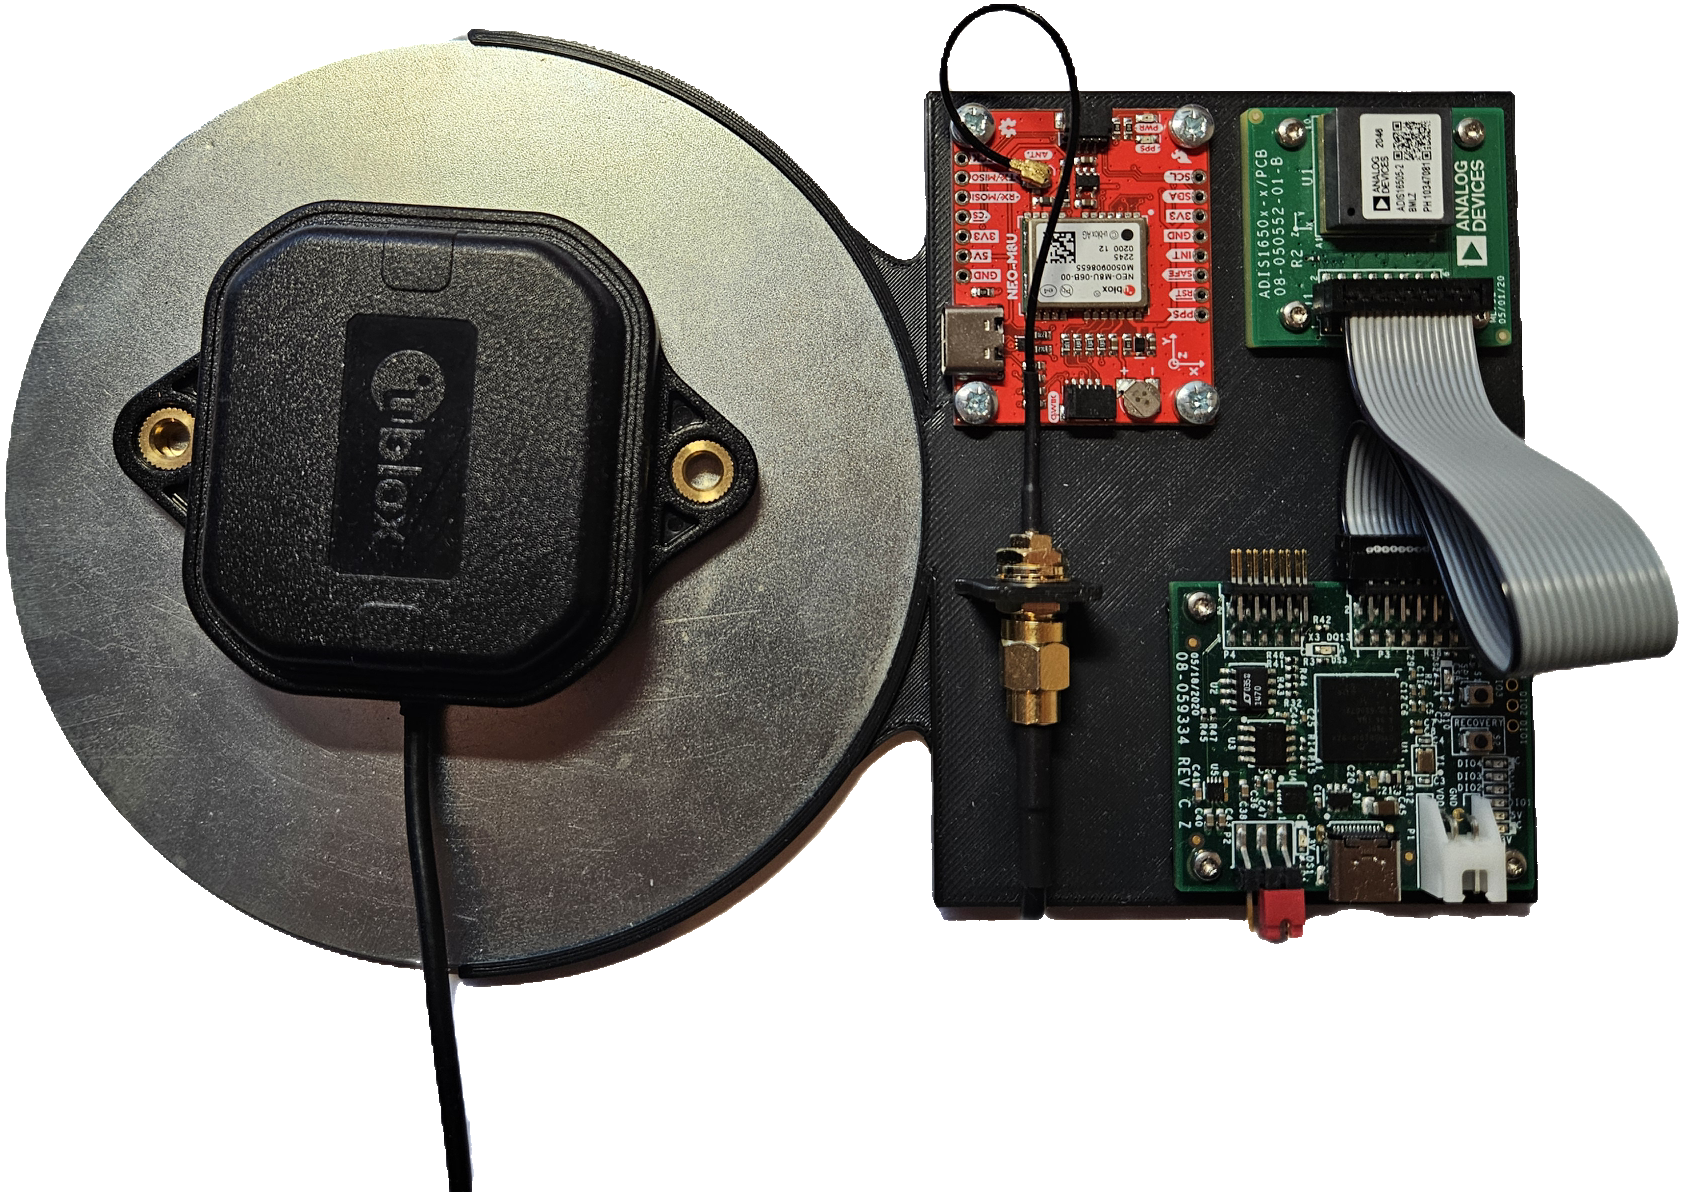
\includegraphics[width=0.8\textwidth]{obrazky/devBoards}
    \caption{Testovací přípravek s vývojovými deskami}
    \label{fig:devBoards}
\end{figure}

\chapter{Realizace hardwaru} \label{hardware}
\begin{figure}[h]
    \centering
    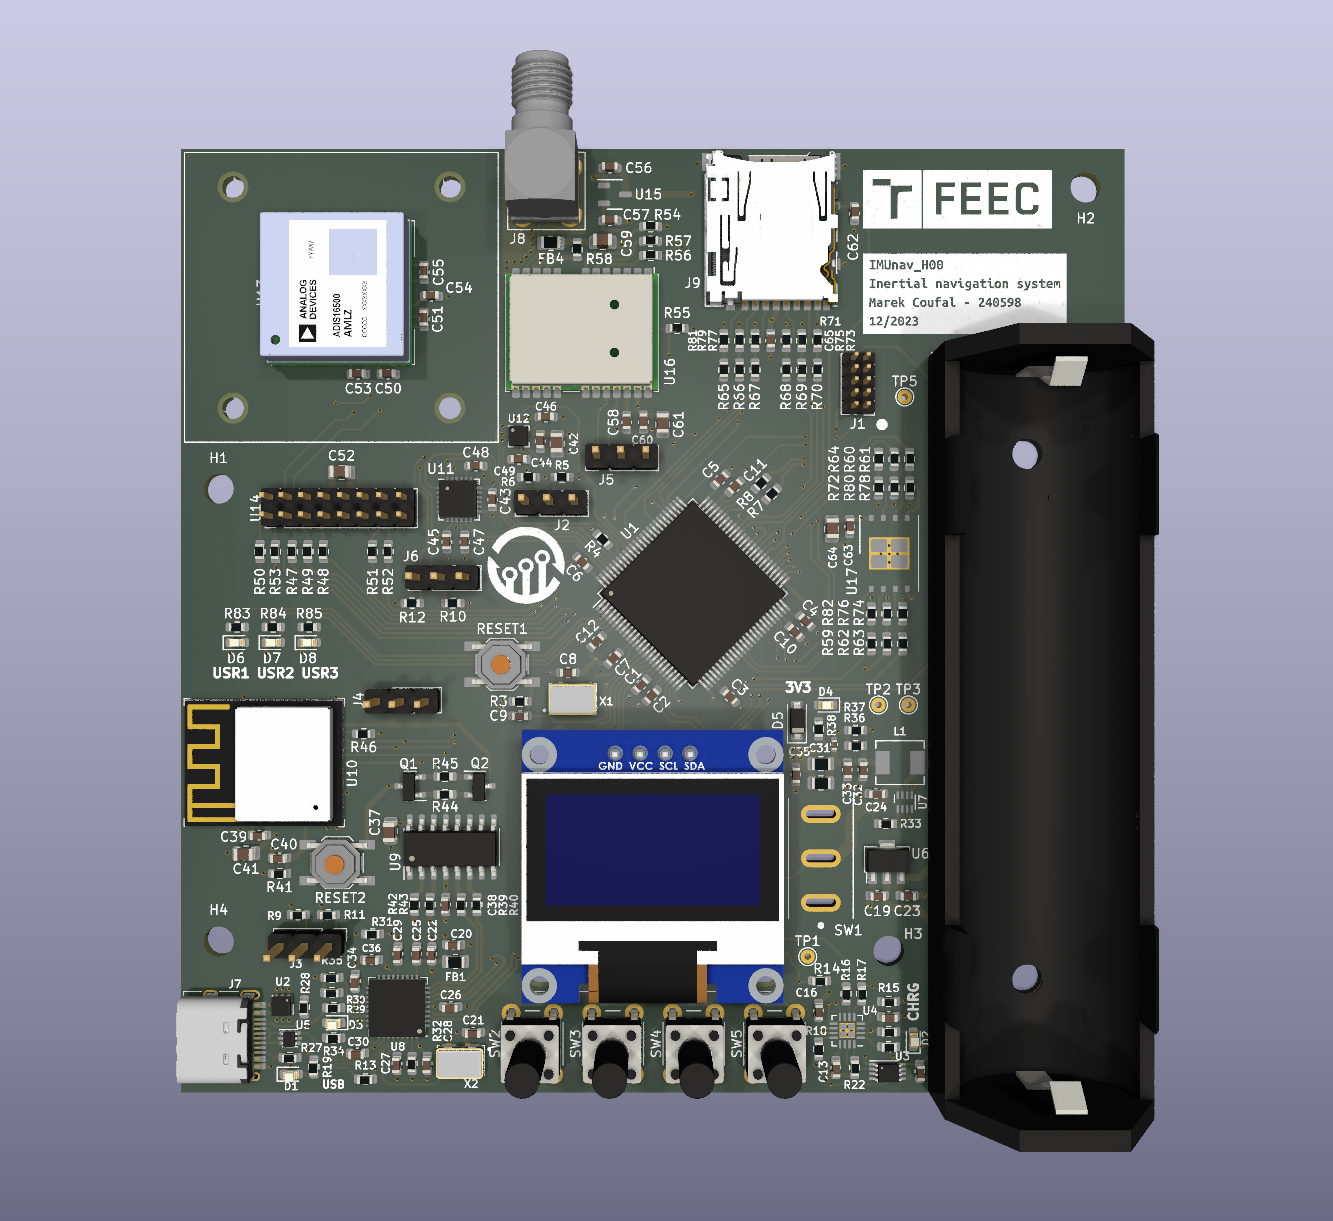
\includegraphics[width=\textwidth]{KiCad/3Dboard}
    \caption{3D model navržené DPS}
    \label{fig:3Dboard}
\end{figure}

Schéma i DPS byla navržena v programu KiCad. V příloze \ref{schemaApp} je schéma inerciální jednotky rozdělené do několika logických bloků. Příloha \ref{placementApp} obsahuje pohled na osazení součástek vrchní vrstvy a přílohy \ref{TopApp} až \ref{BottomApp} obsahují nákres jednotlivých vrstev mědi. Na obrázku \ref{fig:3Dboard} je vygenerovaný 3D model DPS.

Inerciální jednotka je realizována jako 4vrstvá deska plošných spojů o velikosti $ 100 \times 100 $ mm s uspořádáním vrstev popsaném v tabulce \ref{table:signalStackup}.
\begin{table}[h!]
\caption{Signálové uspořádání vrstev na DPS.} 
\centering

\begin{tabular}{|c|c|}
\hline 
Vrstva mědi & Využití \\ 
\hline 
\hline 
Horní & Vysokorychlostní signály \\ 
\hline 
1. vnitřní & Společná zem \\ 
\hline 
2. vnitřní & Napájení \\ 
\hline 
Dolní & Signály \\ 
\hline 
\end{tabular} 


\label{table:signalStackup}
\end{table} 

Typ a tloušťky substrátu DPS byly vybrány v konfiguraci JLC04161H-7628, jejich mechanické uspořádání a dielektrické vlastnosti jsou popsané v tabulce \ref{table:materialStackup}. Pomocí kalkulačky výrobce byly vypočteny potřebné hodnoty požadovaných šířek a mezer spojů mikropáskového vedení pro impedanci \SI{50}{\ohm} a \SI{90}{\ohm}. Hodnoty pro vedení o impedanci \SI{50}{\ohm} byly použity při návrhu cest mezi GPS modulem a SMA anténou. Šírka a vzdálenost diferenciálního páru o impedanci \SI{90}{\ohm} byla použita při návrhu USB části zapojení.
\begin{table}[ht]
\centering

\begin{tabular}{|c|c|c|}
\hline 
Typ materiálu & Tloušťka (mm) & Relativní permitivita $ \epsilon_{r} $(-) \\ 
\hline 
\hline 
Vrchní vrstva mědi & 0,0350 & 1 \\ 
\hline 
Prepreg 7628 & 0,2104 & 4,4 \\ 
\hline 
1. vnitřní vrstva mědi & 0,0152 & 1 \\ 
\hline 
Jádro & 1,065 & 4,6 \\ 
\hline 
2. vnitřní vrstva mědi & 0,0152 & 1 \\ 
\hline 
Prepreg 7628 & 0,2104 & 4,4 \\ 
\hline 
Spodní vrstva mědi & 0,0350 & 1 \\ 
\hline 
\end{tabular} 

\caption{Uspořádání měděných a izolačních vrstev DPS JLC04161H-7628} 
\label{table:materialStackup}
\end{table} 


Většina pouzder pasivních součástek byla vybrána o velikosti 0603, což by mělo poskytovat dostatečný kompromis mezi velikostí výsledné desky a možností ruční výměny součástky pro případné opravy na prvním prototypu. Prototypová deska je také opatřena měřícími body na napájecích větvích a konektorovými hřebínky na digitálních komunikacích pro možnost připojení osciloskopu, nebo logického analyzátoru na odposlouchávání komunikace mezi MCU a jednotlivými senzory. 



